\section{问题二模型的建立与求解}
  \subsection{数据分析}
  我们画出部分特征数据的分布,得到结果如下图所示。从图中我们可以看出,不同版本GCC编译器生成的汇编文件对于操作码、寄存器、Bigram与block数量存在一定的差异,而这也正是我们去判断编译器版本的重要依据。
  \begin{figure}[H]
      \centering
      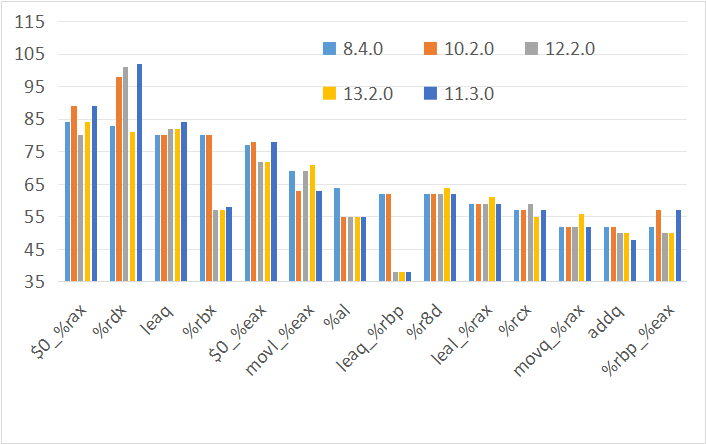
\includegraphics[width=1\linewidth]{hist.png}
      \caption{Enter Caption}
      \label{fig:enter-label}
  \end{figure}

  
计算各个特征与标签的皮尔逊相关系数(Pearson Correlation Coefficient),该系数可以用来衡量适用于衡量两个连续变量之间的线性关系,皮尔逊相关系数的计算公式为
\begin{equation}
\rho_{X,Y} = \frac{\text{cov}(X, Y)}{\sigma_X \sigma_Y}
\label{eq:correlation}
\end{equation}

其中,协方差 \(\text{cov}(X, Y)\) 的计算公式为:
\begin{equation}
\text{cov}(X, Y) = \frac{1}{n} \sum_{i=1}^{n} (X_i - \mu_X)(Y_i - \mu_Y)
\label{eq:covariance}
\end{equation}

标准差 \(\sigma_X\) 和 \(\sigma_Y\) 的计算公式为:
\begin{equation}
\sigma_X = \sqrt{\frac{1}{n} \sum_{i=1}^{n} (X_i - \mu_X)^2}
\label{eq:stddev_x}
\end{equation}
\begin{equation}
\sigma_Y = \sqrt{\frac{1}{n} \sum_{i=1}^{n} (Y_i - \mu_Y)^2}
\label{eq:stddev_y}
\end{equation}

均值 \(\mu_X\) 和 \(\mu_Y\) 的计算公式为:
\begin{equation}
\mu_X = \frac{1}{n} \sum_{i=1}^{n} X_i
\label{eq:mean_x}
\end{equation}
\begin{equation}
\mu_Y = \frac{1}{n} \sum_{i=1}^{n} Y_i
\label{eq:mean_y}
\end{equation}

  \begin{figure}[H]
      \centering
      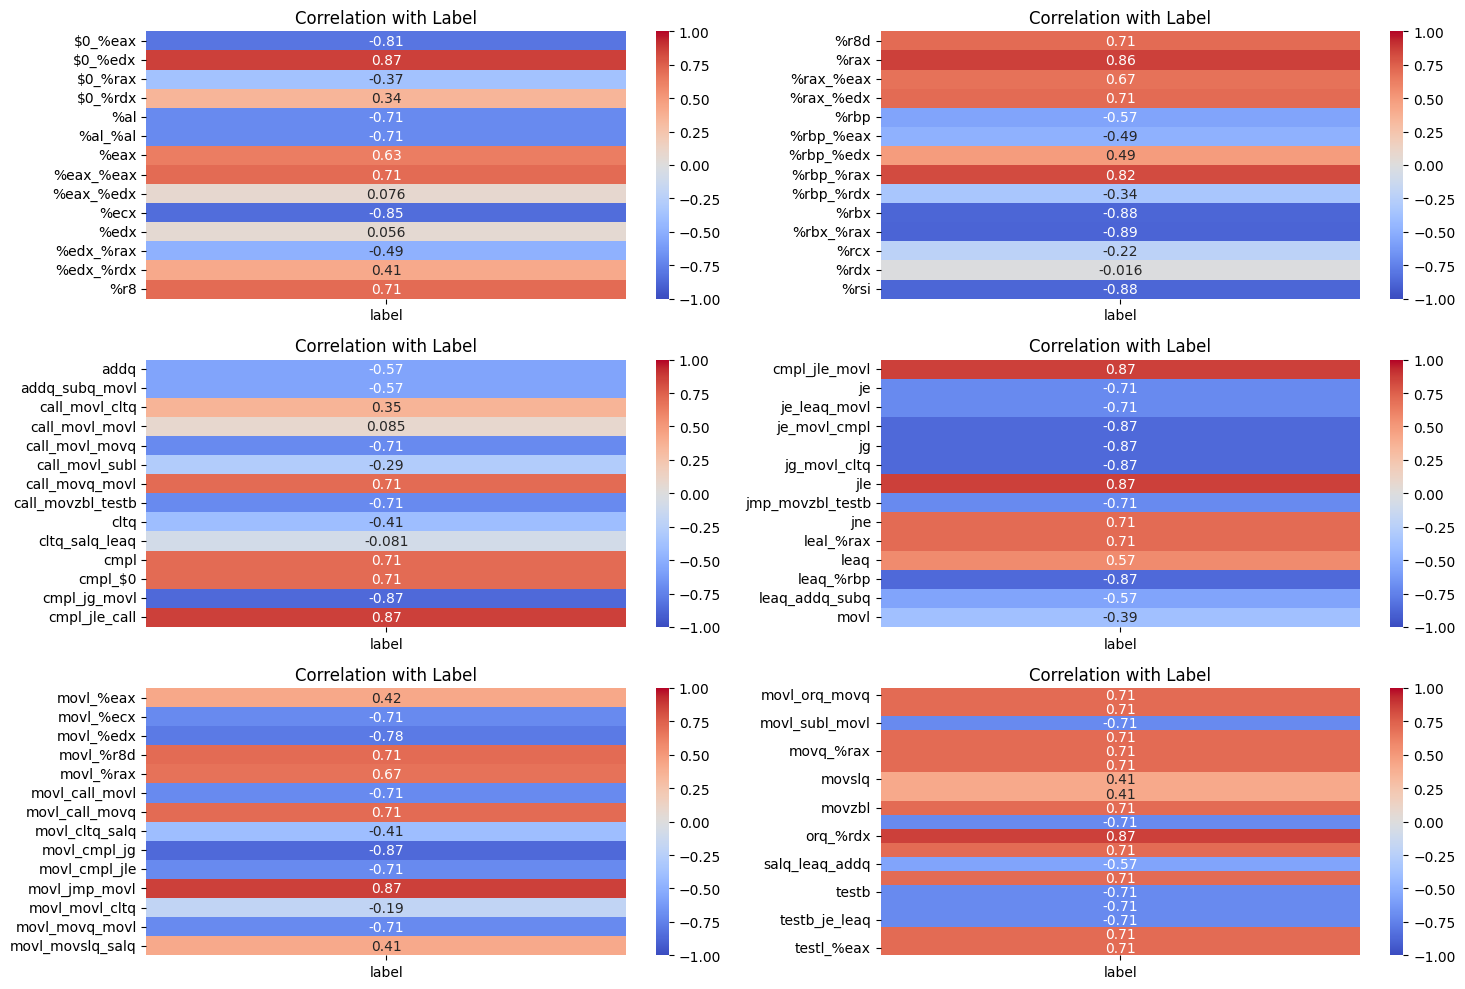
\includegraphics[width=1\linewidth]{corr.png}
      \caption{特征与标签的相关系数}
      \label{fig:enter-label}
  \end{figure}
得到的结果如图所示,虽然图片中部分特征的相关系数较高,但是我们进行了统计显著性检验。我们设原假设$H_0$是“两个变量之间不存在线性关系”,备择假设$H_1$是“两个变量之间存在线性关系”.

我们使用t 统计量来进行相关系数检验。t 统计量的计算公式为:
\begin{equation}
t = \frac{r \sqrt{n - 2}}{\sqrt{1 - r^2}}
\label{eq:t}
\end{equation}
其中:
\begin{itemize}
    \item \(r\) 是计算得到的 Pearson 相关系数。
    \item \(n\) 是样本量。
    \item t 统计量服从自由度为 \(n - 2\) 的 t 分布。
\end{itemize}
计算得到 t 统计量后,可以通过查找 t 分布表或使用计算工具来找到对应的 p 值。p 值是与 t 统计量对应的累积概率值,表示在原假设为真的情况下,t 统计量出现当前值或更极端值的概率。对于p值的解释是:
\begin{itemize}
    \item \textbf{低 p 值(通常 < 0.05)}:意味着在原假设为真的情况下,观察到当前相关系数的概率非常低,因此我们有理由拒绝原假设,认为相关系数是显著的。
    \item \textbf{高 p 值(通常 ≥ 0.05)}:意味着在原假设为真的情况下,观察到当前相关系数的概率较高,因此我们无法拒绝原假设,认为相关系数可能不是显著的。
\end{itemize}
我们可以从图中看到几乎所有的特征属性的$p$值都大于显著性水平 
α=0.05,则不拒绝原假设,认为相关系数可能是由于随机误差引起的,不具有统计显著性。
\begin{figure}[H]
    \centering
    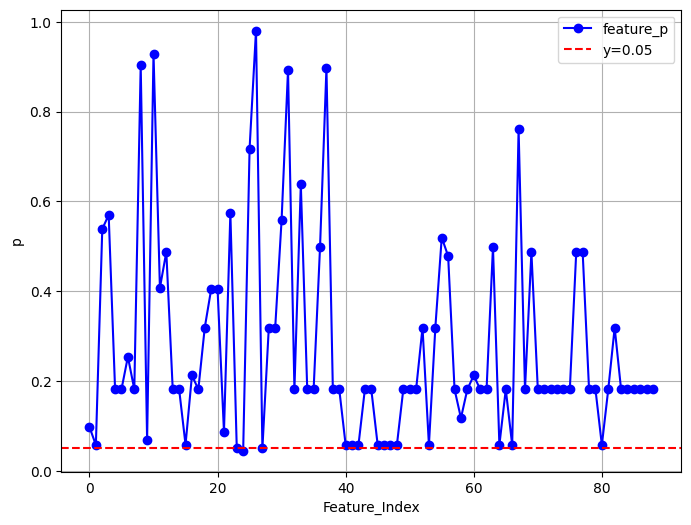
\includegraphics[width=1\linewidth]{p.png}
    \caption{统计显著性水平}
    \label{fig:enter-label}
\end{figure}
 
  
  因此我们接着计算了特征属性与标签的互信息。互信息衡量了两个随机变量之间的“信息共享”量。如果两个随机变量 $X$ 和 
$Y$ 是独立的,那么它们之间的互信息为零,表示知道一个变量不会提供关于另一个变量的任何信息。如果互信息较大,则表示两个变量之间有较强的依赖关系。
 \begin{figure}[H]
      \centering
      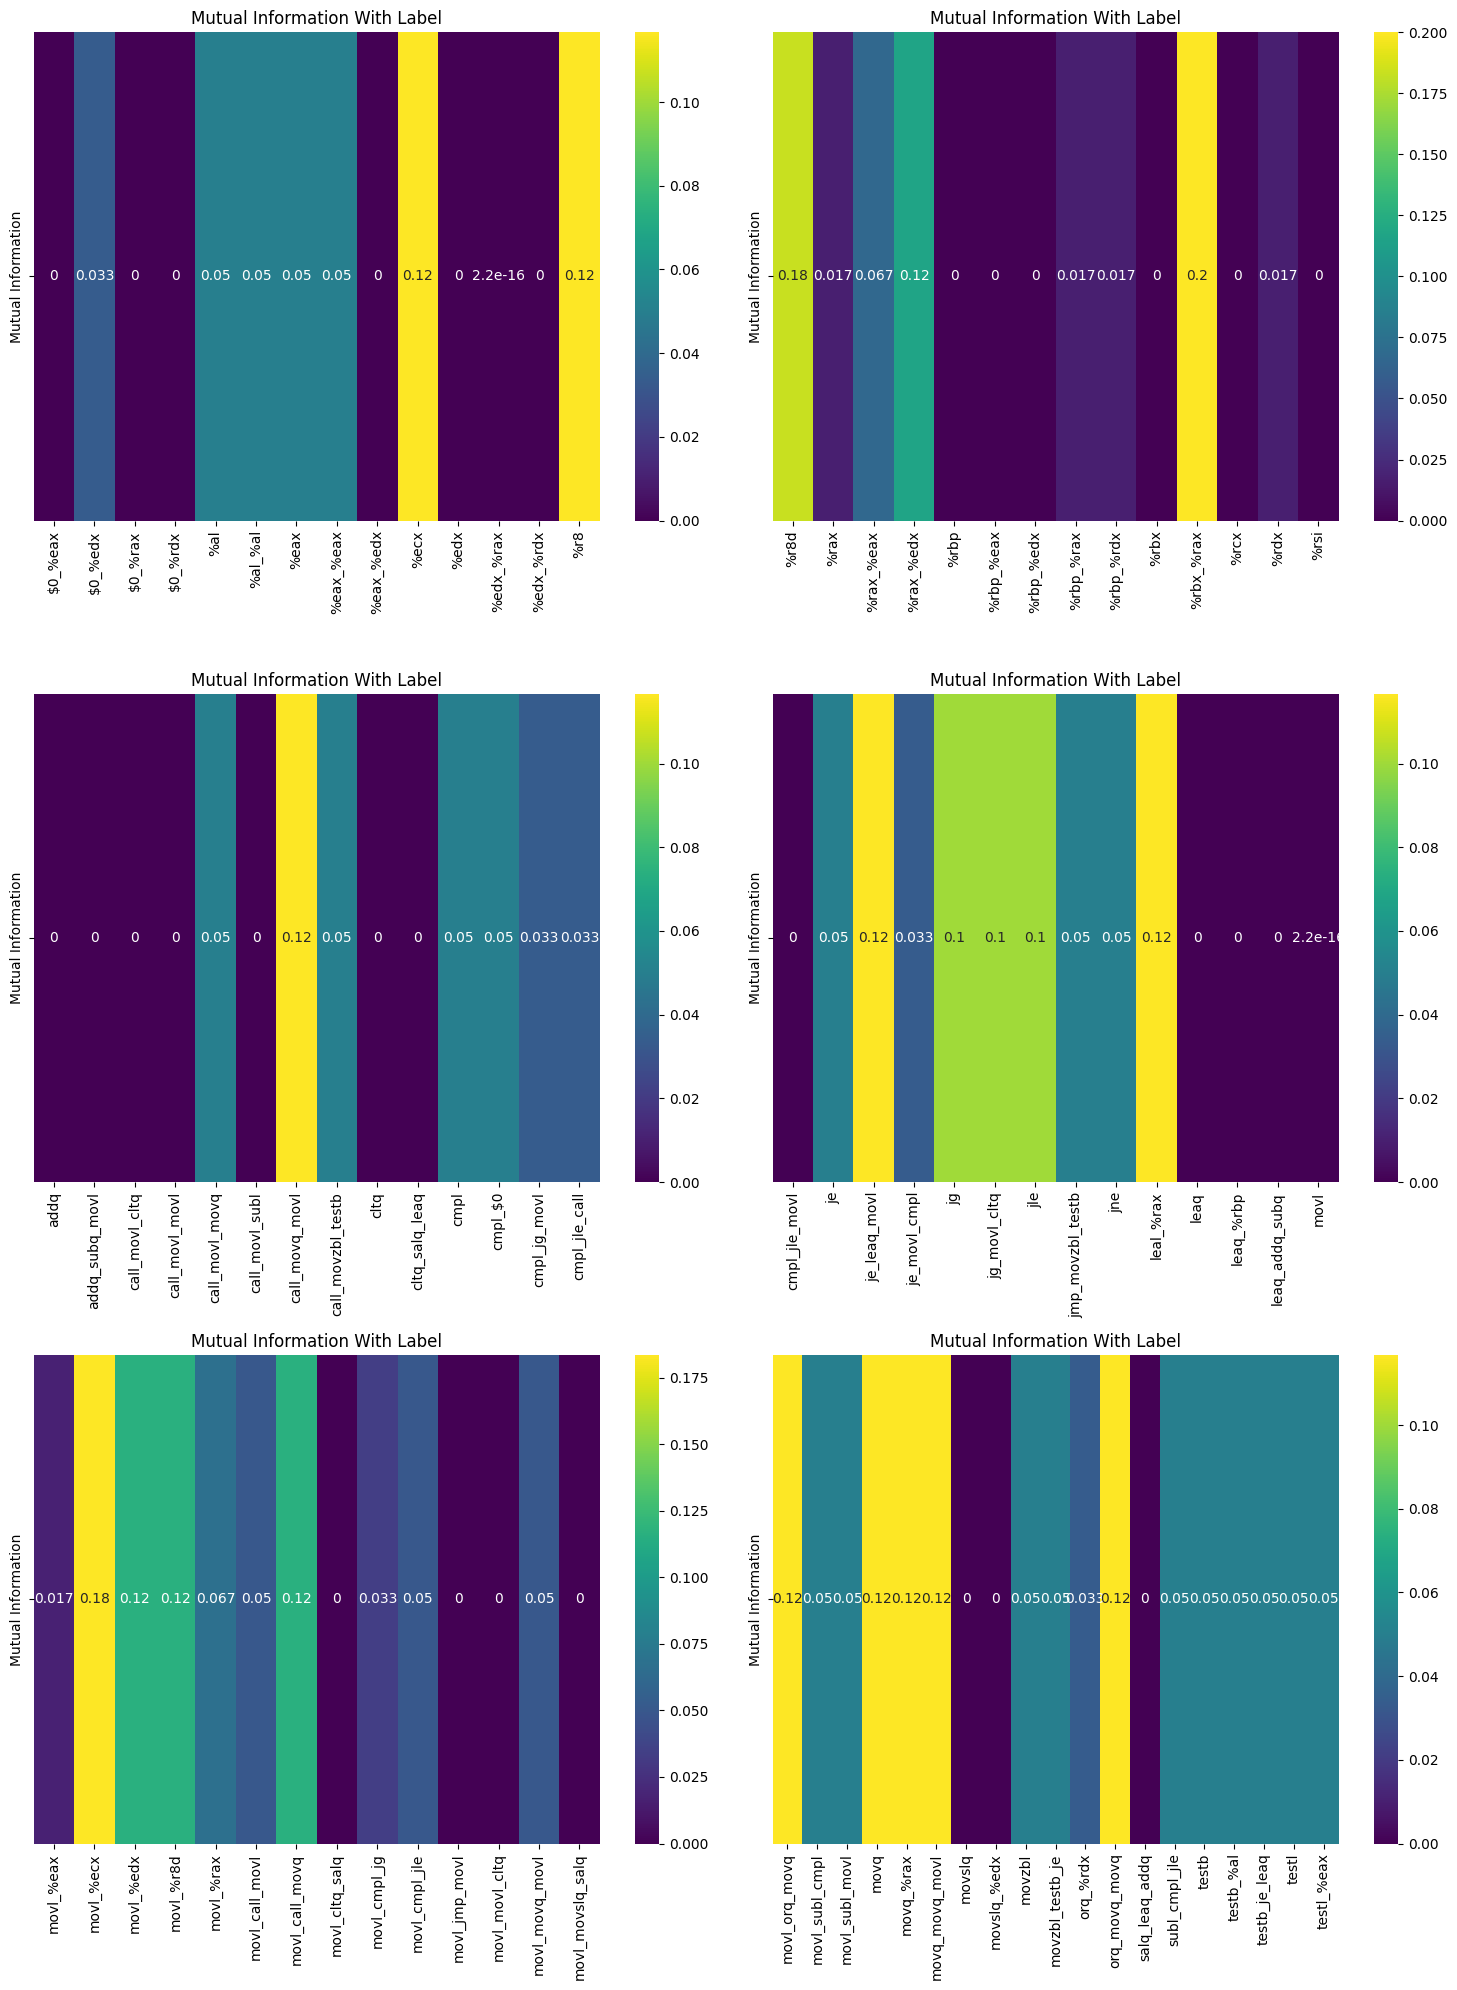
\includegraphics[width=1\linewidth]{Information.png}
      \caption{特征与标签的互信息}
      \label{fig:enter-label}
  \end{figure}
对于两个离散随机变量 \(X\) 和 \(Y\),互信息定义为:
\begin{equation}
I(X; Y) = \sum_{y \in Y} \sum_{x \in X} p(x, y) \log \left(\frac{p(x, y)}{p(x) p(y)}\right)
\label{eq:mutual_information}
\end{equation}

互信息还可以通过熵来表示:
\begin{equation}
I(X; Y) = H(X) + H(Y) - H(X, Y)
\label{eq:mutual_information_entropy}
\end{equation}

其中,各个熵的计算公式为:
\begin{equation}
H(X) = -\sum_{x \in X} p(x) \log p(x)
\label{eq:entropy_x}
\end{equation}

\begin{equation}
H(Y) = -\sum_{y \in Y} p(y) \log p(y)
\label{eq:entropy_y}
\end{equation}

\begin{equation}
H(X, Y) = -\sum_{x \in X} \sum_{y \in Y} p(x, y) \log p(x, y)
\label{eq:joint_entropy}
\end{equation}
从图中我们可以得到如下信息:
\begin{itemize}
    \item 高互信息的特征:互信息值高的特征(如 '\%edx\_\%eax'、'\%r8d'、'cmp\_jle\_movl' 等)在图中以黄色或绿色显示,这些特征是我们在模型中特别需要关注的,因为它们对标签具有较高的预测能力。
    \item 低互信息或零互信息的特征:互信息值为零或接近零的特征对标签几乎没有贡献,可以考虑在特征选择过程中进行剔除或降低其权重,以简化模型。
    \item 互信息的分布:从图中可以看出,互信息较高的特征集中在一些特定的寄存器组合或指令组合上,这表明这些组合对于模型预测特别重要。基于此,我们可以重点关注这些特征,并在模型训练中对其进行优化。
\end{itemize}

因此,我们根据数据分析以及阅读的论文,猜想特征属性与编译器版本之间存在的关系应该是非线性关系。而由于我们的数据是连续值,且考虑到不同源代码生成的汇编文件可能存在不同的特征属性,所以我们的模型还要求支持对含有缺失值的数据进行预测,综合考量,我们决定使用Gini决策树,该决策树可以很好的支持上述特性。
    \subsection{模型说明}
    \subsubsection{Gini系数的计算}
Gini系数是衡量数据集中样本纯度的指标。对于给定的样本集合 \(D\),Gini系数可以表示为:
\begin{equation}
Gini(D) = 1 - \sum_{i=1}^{C} p_i^2
\end{equation}
其中:
\begin{itemize}
  \item \(p_i\) 是样本集中第 \(i\) 类的样本比例(即属于第 \(i\) 类的样本数量占总样本数量的比例)。
  \item \(C\) 是类别的数量。
\end{itemize}





\subsubsection{连续属性划分点t的确定}

\paragraph{排序连续属性的值}
对于一个连续属性 \(A\),首先对所有样本的该属性值进行排序。假设排序后的值为 \(a_1, a_2, \dots, a_n\),其中 \(a_i\) 是第 \(i\) 个样本在属性 \(A\) 上的取值,并且满足 \(a_1 \leq a_2 \leq \dots \leq a_n\)。

\paragraph{候选划分点的确定}
候选划分点 \(t_i\) 通常选在两个相邻样本值的中间,即:
\begin{equation}
t_i = \frac{a_i + a_{i+1}}{2}, \quad i = 1, 2, \dots, n-1
\end{equation}

\paragraph{计算每个划分点的Gini指数}
对于每个候选划分点 \(t_i\),将数据集 \(D\) 分为两个子集 \(D_{\text{left}}\) 和 \(D_{\text{right}}\):
\begin{equation}
D_{\text{left}} = \{x \in D \mid A(x) \leq t_i\}
\end{equation}
\begin{equation}
D_{\text{right}} = \{x \in D \mid A(x) > t_i\}
\end{equation}

然后计算基于划分点 \(t_i\) 的Gini指数:
\begin{equation}
Gini(D, A, t_i) = \frac{|D_{\text{left}}|}{|D|} Gini(D_{\text{left}}) + \frac{|D_{\text{right}}|}{|D|} Gini(D_{\text{right}})
\end{equation}

\paragraph{选择最优划分点}
最优划分点 \(t^*\) 是使得Gini指数最小的划分点:
\begin{equation}
t^* = \arg\min_{t_i} Gini(D, A, t_i)
\end{equation}

通过此方法,我们得到了最优的划分点 \(t^*\),并将其用于决策树的构建。






\subsubsection{处理连续属性}
对于连续属性 \(A\),通过划分点 \(t\) 将样本集 \(D\) 划分为两个子集:\(D_{\text{left}}\) 和 \(D_{\text{right}}\),分别表示小于等于 \(t\) 和大于 \(t\) 的样本集。划分后的Gini指数为:
\begin{equation}
Gini(D, A, t) = \frac{|D_{\text{left}}|}{|D|} Gini(D_{\text{left}}) + \frac{|D_{\text{right}}|}{|D|} Gini(D_{\text{right}})
\end{equation}
其中:
\begin{itemize}
  \item \(|D_{\text{left}}|\) 和 \(|D_{\text{right}}|\) 是两个子集的样本数量。
  \item \(Gini(D_{\text{left}})\) 和 \(Gini(D_{\text{right}})\) 分别是两个子集的Gini系数。
  \item \(|D|\) 是样本集 \(D\) 的总样本数量。
\end{itemize}

\subsubsection{处理缺失值}
对于属性 \(A\) 存在缺失值的情况,假设缺失值比例为 \(p_{\text{missing}}\),则Gini系数可以表示为:
\begin{equation}
Gini(D, A) = (1 - p_{\text{missing}}) \times Gini(D_{\text{not-missing}}, A) + p_{\text{missing}} \times Gini(D_{\text{missing}})
\end{equation}
其中:
\begin{itemize}
  \item \(D_{\text{not-missing}}\) 是属性 \(A\) 有值的样本集。
  \item \(D_{\text{missing}}\) 是属性 \(A\) 缺失值的样本集。
  \item \(Gini(D_{\text{not-missing}}, A)\) 和 \(Gini(D_{\text{missing}})\) 分别是有值样本集和缺失值样本集的Gini系数。
\end{itemize}

\subsubsection{选择最优划分}
在考虑了所有可能的划分点 \(t\) 以及缺失值的影响后,选择使得Gini指数最小的划分点作为最终的划分点,以确保在当前节点上的样本被分成更加纯净的子集。

\subsubsection{构建树结构}
在找到最优划分后,决策树会在此处创建一个分裂节点,并将数据集分成左右子集。然后递归地对每个子集重复上述步骤,直到满足停止条件为止。

\subsection{模型建立}
Gini决策树的伪代码如下:
\begin{algorithm}[H]
    \caption{决策树构建算法}
    \label{alg:decision_tree}
    \begin{algorithmic}
        \REQUIRE 数据集 $D$,属性集 $A$,停止条件
        \ENSURE 决策树

        \STATE \textbf{函数} \texttt{BuildTree}($D$, $A$):
        \STATE \quad \textbf{If} 所有样本都属于同一类 \textbf{Then}
        \STATE \quad \quad 将当前节点标记为该类,返回
        \STATE \quad \textbf{If} 属性集为空或满足停止条件 \textbf{Then}
        \STATE \quad \quad 将当前节点标记为样本中最多的类,返回
        \STATE \quad \textbf{For each} 属性 $A_i \in A$ \textbf{Do}
        \STATE \quad \quad \textbf{If} $A_i$ 是连续属性 \textbf{Then}
        \STATE \quad \quad \quad 对 $A_i$ 的值进行排序
        \STATE \quad \quad \quad 计算每个候选划分点 $t_i = \frac{a_i + a_{i+1}}{2}$
        \STATE \quad \quad \quad 对每个候选划分点 $t_i$ 计算 Gini 指数
        \STATE \quad \quad \textbf{Else If} $A_i$ 有缺失值 \textbf{Then}
        \STATE \quad \quad \quad 计算 Gini 指数,考虑缺失值比例 $p_{\text{missing}}$
        \STATE \quad \quad \textbf{Else}
        \STATE \quad \quad \quad 计算每个可能划分的 Gini 指数
        \STATE \quad 选择使 Gini 指数最小的属性 $A^*$ 及其最优划分点 $t^*$
        \STATE \quad 将当前节点标记为 $A^*$ 的分裂节点
        \STATE \quad 根据划分点 $t^*$ 将样本集 $D$ 分为 $D_{\text{left}}$ 和 $D_{\text{right}}$
        \STATE \quad 递归调用 \texttt{BuildTree}($D_{\text{left}}$, $A$) 和 \texttt{BuildTree}($D_{\text{right}}$, $A$)
        
        \STATE \textbf{End Function}
    \end{algorithmic}
\end{algorithm}
基于伪代码,我们构建了一颗Gini决策树,如下图所示:
\begin{figure}[H]
    \centering
    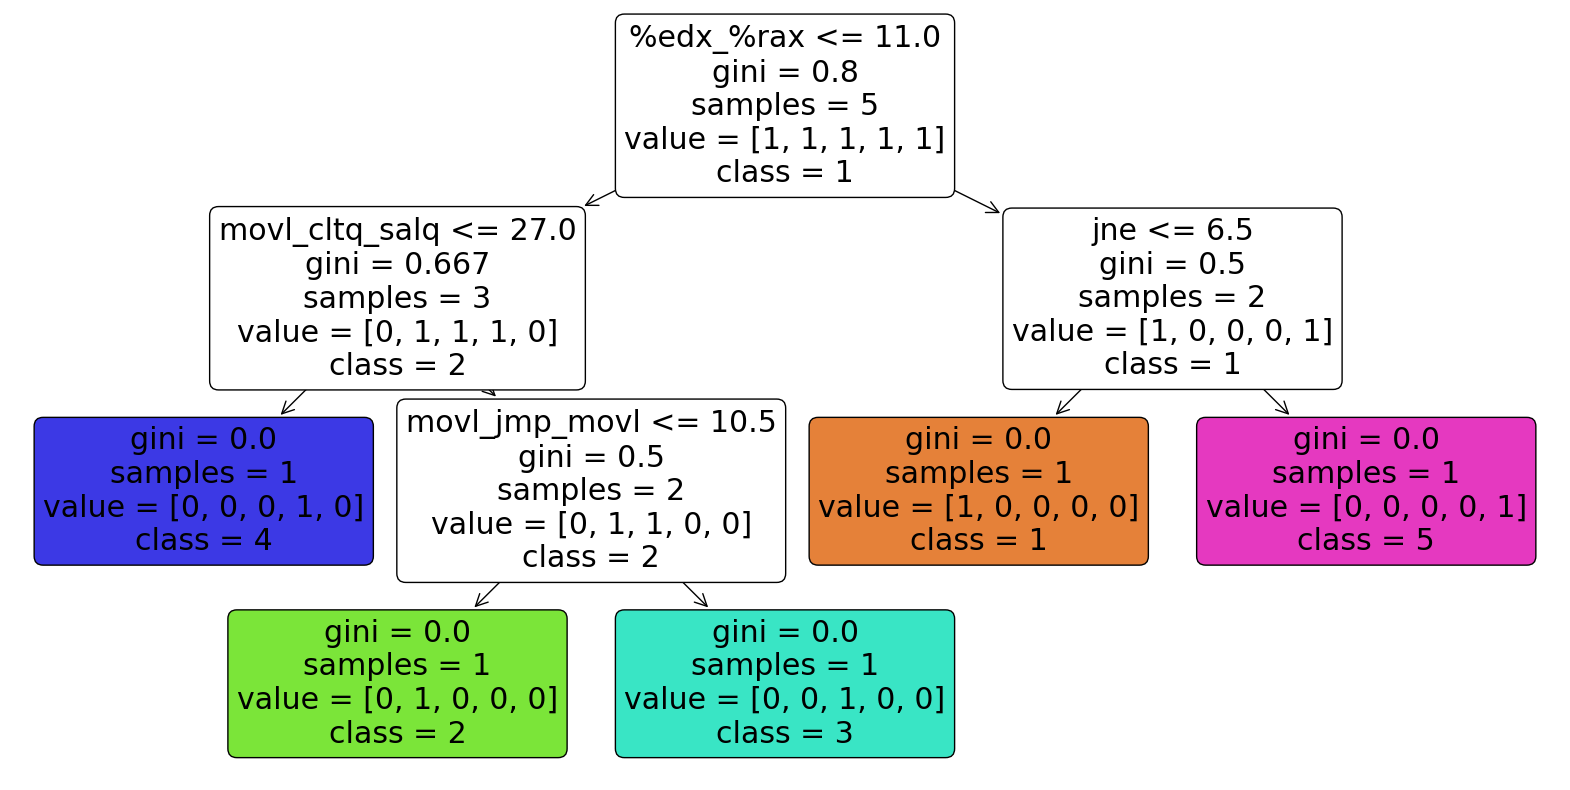
\includegraphics[width=1\linewidth]{Ginitree.png}
    \caption{Gini决策树}
    \label{fig:enter-label}
\end{figure}
